\documentclass[11pt,a4paper]{article}
\usepackage{amsmath}
\usepackage{amsfonts}
\usepackage{amssymb}
\usepackage{makeidx}
\usepackage{graphicx}
\usepackage{wrapfig}
\usepackage{enumerate}
\usepackage{pdfpages}
\usepackage{tocloft}
\usepackage{setspace}
\usepackage{mathtools}
\usepackage{hyperref}
\definecolor{linkcolour}{rgb}{0,0.2,0.6} % Link color
\hypersetup{colorlinks,breaklinks,urlcolor=linkcolour,linkcolor=linkcolour}

\usepackage[left=2cm,right=2cm,top=1.5cm,bottom=1.5cm]{geometry}

\usepackage{xcolor}

\usepackage{color,soul}
\usepackage{fontspec}
\setmainfont{Cambria}

\usepackage{caption}
\captionsetup[figure]{font=small, labelfont={bf}}
\captionsetup[table]{font=small, labelfont={bf}}

\usepackage{float}
\usepackage{multirow}
\usepackage{longtable}

\usepackage[nottoc]{tocbibind}

\newcommand{\spa}{\vspace{1.25em}}
\newcommand{\noi}{\noindent}
\def\dul#1{\underline{\underline{#1}}}
\def\cpt#1#2{{\begin{center}\small\textbf{\textcolor{blue}{Figure #1:}} #2\end{center}}}
\def\tt#1{\texttt{#1}}

% for dots in the content
\usepackage{tocloft}
\renewcommand{\cftsecleader}{\cftdotfill{\cftdotsep}}

\begin{document}
	\begin{titlepage} 
		\begin{center}
		\large{ASSIGNMENT 2}\\
		\vspace{2em}
		\large {CS5691 Pattern Recognition and Machine Learning}
		\vspace{3em}
		
		\rule{0.9\linewidth}{0.5mm} \\[0.4cm]
	    {\Large{\bfseries{CS5691 Assignment 2}}} \\
	    \rule{0.9\linewidth}{0.5mm} \\[3 em]	
	    
	    Team Members: \\
	    \vspace{0.5em}
	   	\def\arraystretch{1.25}
\begin{tabular}{c l}
	\hline
	BE17B007 & N Sowmya Manojna \\
	PH17B010 & Thakkar Riya Anandbhai \\
	PH17B011 & Chaithanya Krishna Moorthy \\
	\hline
\end{tabular}

		\vspace{1em}

		Indian Institute of Technology, Madras\\    
		
		\vspace{5em}    
	    
	    	
\includegraphics[scale=0.09]{images/iitmlogo.png}
		\end{center}
	\end{titlepage}

{\hypersetup{linkcolor=black}
 \tableofcontents}
\break


\section{Dataset 1A}
\subsection{K-nearest Neighbors Classifier}
\subsubsection{Mathematical Formulation}
\label{sec:1_1}

The K Nearest Neighbor is a statistically non-parametric model that can be used for regression as well as for classification. It assumes that similar things exist in close proximity.  
\noi
Crucial steps in a K-Nearest Neighbor classifier are:
\begin{itemize}
    \itemsep0em
    \item A distance metric is first specified, the most commonly used metric is the euclidean distance:
    \begin{equation}
        d=||\vec{x_1}-\Vec{x_2}||
    \end{equation}
    
    where $||.||$ denotes the norm function. Other commonly used distance metrics are the Manhattan distance and Cosine similarity. For our application, Euclidean distance is used. 
    \item Using the specified distance metric, the distance between the test instance and each training example is evaluated.
    \item The class label that occurs most frequently amongst the nearest $k$ training examples is assigned to the test instance.
\end{itemize}

\noi
Advantages of KNN are:
\begin{itemize}
    \itemsep0em
    \item KNN does not require a training period, it just stores the training dataset and learns from it at the time of making a prediction, hence it is generally much faster than other classification algorithm.
    \item Since the algorithm does not require prior training, new data points can be added seamlessly. 
    \item Easy to implement,the number of parameters are just two: $k$ and the distance metric to be used.
\end{itemize}

\noi
Disadvantages of KNN are:
\begin{itemize}
    \itemsep0em
    \item Computationally expensive for large datasets or high number of features, since the distance is evaluated between test point and all the points in the training dataset. 
    \item Sensitive to noisy data and outliers. Generally, increasing the value of $k$ reduces the effect of noise.
\end{itemize}

\subsubsection{Pre-Processing}
\label{sec:1_1_1}
The dataset 1A has 4 unique class labels - $[0.0, 1.0, 2.0, 3.0]$ as shown in \autoref{fig:1A_decreg_KNN}. Number of examples corresponding to each class label is $200$.
The train dataset is of dimension $(800,3)$ while the CV dataset is of dimension $(120,3)$. The third column in both datasets is the class label, while the first two columns are the real valued feature vectors - $x_1$ and $x_2$.
\begin{itemize}
    \itemsep0em
    \item There are no null values in the datasets. 
    \item The rows of dev dataset are shuffled and further split into cross-validation and test data in the ratio of 70:30
    \item Range of $x_1$ is $(-11,11)$ and range of $x_2$ is $(-12,7)$. Since the ranges are almost similar, no feature scaling is required.  
\end{itemize}

\subsubsection{Model performance across $k$}
The model was evaluated for $k$ values: $[1,7,15]$. We find that irrespective of the value of hyperparameter $k$, the model obtained an accuracy of 100 over training data, cross-validation data as well as the test data. \\

\noi
Since model performance is best irrespective of $k$, the accuracy table, confusion matrix and decision boundary plot are all evaluated using $k=1$ as to minimize the run time.\\

\noi
The accuracy table and confusion matrix are: 
\input{tables/acc_1A_KNN}

\begin{figure}[H]
    \centering
    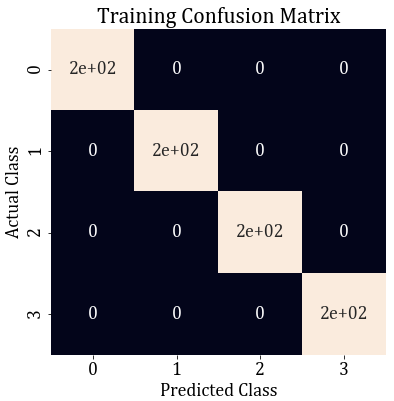
\includegraphics[scale=0.55]{images/1A/1A_cm_knn_train.png}
    \hspace{2em}
    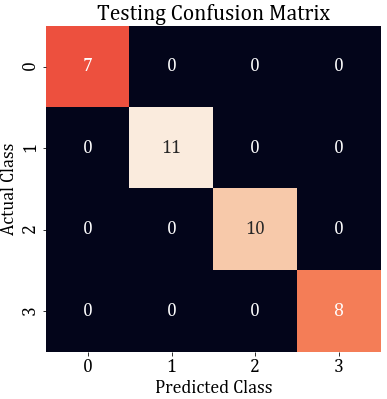
\includegraphics[scale=0.55]{images/1A/1A_cm_knn_test.png}
    \caption{Confusion matrix for $k=1$, Train and Test dataset on left and right respectively}
    \label{fig:1A_cm_KNN}
\end{figure}

\subsubsection{Decision Region Plot}
\begin{figure}[H]
    \centering
    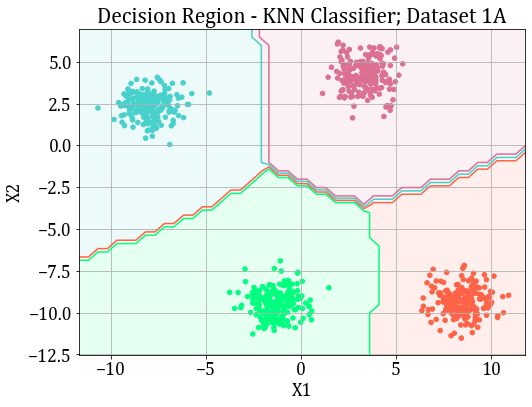
\includegraphics[scale=0.7]{images/1A/1A_knn_decision_region.png}
    \caption{Decision region superimposed with training dataset}
    \label{fig:1A_decreg_KNN}
\end{figure}

The decision boundary obtained (with $k=1$) is linear in form. 

\break
\subsection{Naive-Bayes classifier with a Gaussian distribution for each class}
\label{naive-bayes}
\subsubsection{Mathematical Formulation}
The Bayes Classifiers are probabilistic classifiers based on the Bayes theorem:

\begin{equation}
\label{eqn nb}
    p(y_{i}|\vec{x})=\frac{p(\vec{x}|y_{i}) \times p(y_{i})}{p(\vec{x})}
\end{equation}\\

\noi
Here,
\begin{itemize}
    \itemsep0em
    \item $p(y_{i})$ : prior probability for $y=y_{i}$.
    \item $p(\vec{x}|y_{i})$ : Class conditional probability density function or class conditional likelihood function.
    \item $p(y_{i}|\vec{x})$ : Posterior probability for $y=y_{i}$ given $\vec{x}$
    \item $p(\vec{x})$ : Evidence or normalization factor
\end{itemize}

\noi
\autoref{eqn nb} can be re-written as:
\begin{equation} \label{normalized_nb}
    p(y_{i}|\vec{x})=\frac{p(\vec{x}|y_{i}) \times p(y_{i})}{\sum_{i}p(\vec{x}|y_{i}) \times p(y_{i})}
\end{equation}\\

\noi
Hence, the probability that $\vec{x}$ belongs to the class $y_{i}$ is $\propto$ $p(\vec{x}|y_{i}) \times p(y_{i})$.\\

\noi
Step-wise approach:
\begin{itemize}
    \itemsep0em
    \item $p(y_{i})$ is calculated from the train dataset, for dataset 1A, we find that all the classes have equal prior probability.
    \item The probability $p(\vec{x}|y_{i})$ can be calculated by various parametric and non-parametric means. For dataset 1A, we use parametric means as described later.
    \item $p(y_{i}|\vec{x})$ is calculated for all the classes using \autoref{normalized_nb}.
    \item The class label with maximum posterior probability is chosen as the class label for $\vec{x}$.
\end{itemize}

\noi
For the discussion that follows for dataset 1A, we assume that $p(\vec{x}|y_{i})$ is given by a gaussian distribution:

\begin{equation}
\label{gaussian}
    p(\vec{x}|y_{i})=\frac{1}{(2\pi)^{d/2}*|C_{i}|^{1/2}}\;\exp{\Big(\frac{-(\vec{x}-\vec{\mu_{i}})^{T}C_{i}^{-1}(\vec{x}-\vec{\mu_{i}})}{2}}\Big)
\end{equation}

\noi
In the above equation: 

\begin{itemize}
    \item $\mu_{i}$ is the mean corresponding to examples in the class $y_{i}$, its dimension is $(d,1)$, where $d$ is the number of features. Hence, if there are $k$ classes, number of parameters to be estimated for mean: $k*d$.
    \item $C_{i}$ is the $(d,d)$ covariance matrix corresponding to the class $y_{i}$. Since it is symmetric, number of parameters to be calculated per class: $\frac{d(d+1)}{2}$. Total parameters for covariance: $\frac{k*d(d+1)}{2}$.
\end{itemize}

\noi
The co-variance matrix and eigen-vectors for each class are calculated and are found to be as follows:
\begin{itemize}
    \item For class y=0.0: 
    $$
    C = 
    \begin{bmatrix}
    0.676 & -0.005 \\
    -0.005 & 0.784 \\
    \end{bmatrix}
    $$
    $$
    eigen-vectors = 
    \begin{bmatrix}
    -0.999 & 0.049 \\
    \end{bmatrix}
    ,
    \begin{bmatrix}
    0.106 & 0.996 \\
    \end{bmatrix}
    $$
    \item For class y=1.0:
    $$
    C = 
    \begin{bmatrix}
    0.731 & 0.022 \\
    0.022 & 0.523 \\
    \end{bmatrix}
    $$
    $$
    eigen-vectors = 
    \begin{bmatrix}
    0.994 & -0.106 \\
    \end{bmatrix}
    ,
    \begin{bmatrix}
    0.106 & 0.994 \\
    \end{bmatrix}
    $$
    \item For class y=2.0:
    $$
    C = 
    \begin{bmatrix}
    0.767 & 0.009 \\
    0.009 & 0.671 \\
    \end{bmatrix}
    $$
    $$
    eigen-vectors = 
    \begin{bmatrix}
    0.996 & -0.090 \\
    \end{bmatrix}
    ,
    \begin{bmatrix}
    -0.090 & 0.996 \\
    \end{bmatrix}
    $$
    \item For class y=3.0:
    $$
    C = 
    \begin{bmatrix}
    0.705 & 0.028 \\
    0.028 & 0.621 \\
    \end{bmatrix}
    $$
    $$
    eigen-vectors = 
    \begin{bmatrix}
    0.957 & -0.289 \\
    \end{bmatrix}
    ,
    \begin{bmatrix}
    0.289 & 0.957 \\
    \end{bmatrix}
    $$
\end{itemize}


\subsubsection{Accuracy table and Confusion Matrix}
We obtain that irrespective of our assumption of the co-variance matrices, the accuracy over train, validation and test set is 1. 
\def\arraystretch{1.25}
\begin{table}[H]
\centering
\begin{tabular}{l l l l l}
\hline
\hline
\textbf{Condition} & \textbf{Train Accuracy} & \textbf{Validation Accuracy} & \textbf{Test Accuracy}\\
\hline
\hline
$C_{i}=C_{j}=\sigma^{2}I$ & 100 & 100 & 100\\
$C_{i}=C_{j}=C$ & 100 & 100 & 100 \\
$C_{i}\neq C_{j}$ & 100 & 100 & 100 \\
\hline
\end{tabular}
\caption{Accuracy table for dataset 1A: Bayes Classifier}
\end{table}

\begin{figure}[H]
    \centering
    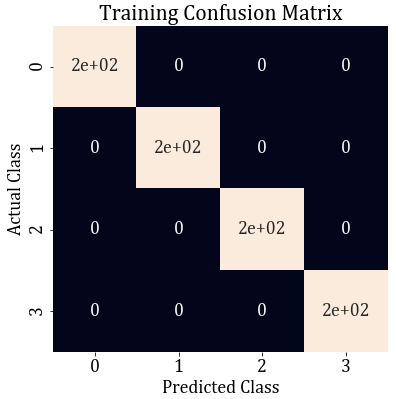
\includegraphics[scale=0.55]{images/1A/1A_cm_nb_train.png}
    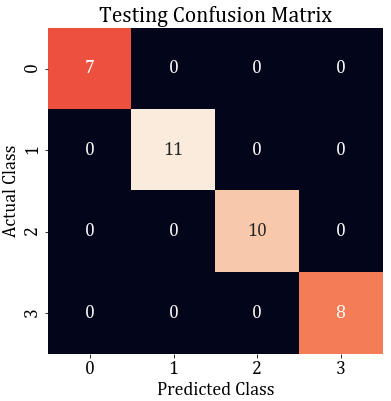
\includegraphics[scale=0.55]{images/1A/1A_cm_nb_test.png}
    \caption{Confusion matrix for train and test data respectively}
    \label{fig:conf_mats}
\end{figure}

\break
\subsubsection{Level curve plots for different cases}
\begin{figure}[H]
    \centering
    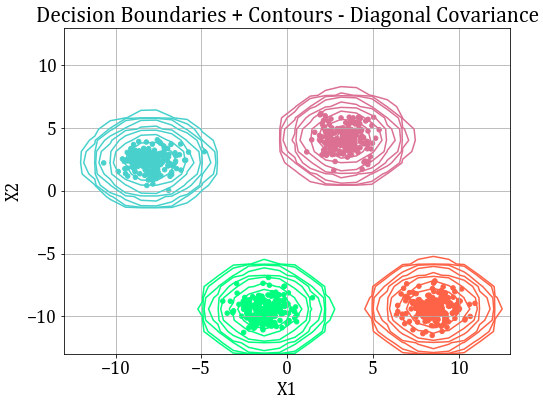
\includegraphics[scale=0.5]{images/1A/1A_contour_case1.png}
    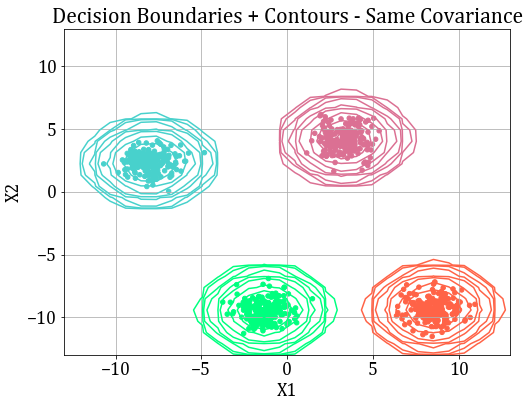
\includegraphics[scale=0.5]{images/1A/1A_contour_case2.png}
    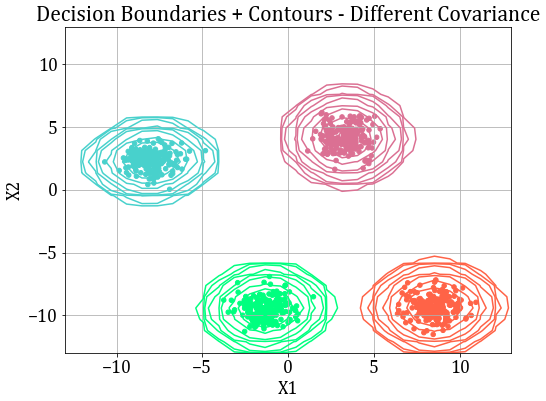
\includegraphics[scale=0.5]{images/1A/1A_contour_case3.png}
    \caption{Contour plots}
    \label{fig:cp_1}
\end{figure}

\subsubsection{Observations} 
\begin{itemize}
    \itemsep0em
    \item For all the three cases, we find that the principal axes of the ellipses are nearly parallel to the coordinate axis. This is because the eigen-vectors are nearly equal to [1,0] and [0,1].
    \item In case a and case b, the length of principal axes are same across all classes. 
    \item In case c, since we have used different co-variance matrix, the length of principal axes are scaled accordingly for all classes.
\end{itemize}

\subsubsection{Decision Boundary plot for Naive Bayes Classifier}
\begin{figure}[H]
    \centering
    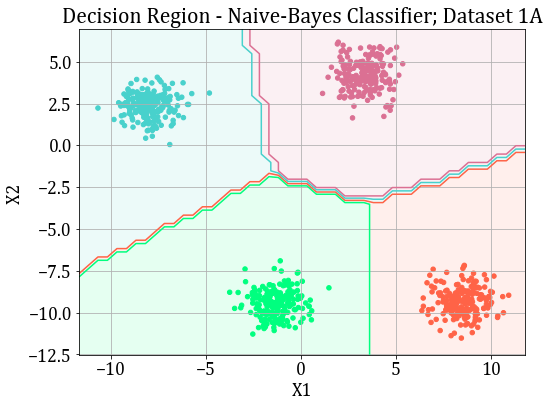
\includegraphics[scale=0.6]{images/1A/1A_nb_case1_decisionregion.png}
    \caption{Decision boundary plot}
    \label{fig:db1}
\end{figure}

\noi

\break
\section{Dataset 1B}
\subsection{K Nearest Neighbor Classifier} 

Similar to \autoref{sec:1_1}, K Nearest Neighbor classifier is used to predict class labels for dataset 2A. \\

\noi
The dataset 1B has 3 unique class labels - $[0.0, 1.0, 2.0]$ and non-linearly separable. The train dataset is of dimension $(800,3)$ while the dev dataset is of dimension $(90,3)$. Similar preprocessing steps are performed as in \autoref{sec:1_1_1}.

\subsubsection{Model performance across $k$}
Unlike dataset 1A, we observe that the accuracy over validation set decreases on increasing the value of hyper-parameter $k$. This happens because the dataset 1B is non-linear, a higher $k$ value includes points from other class labels resulting in mis-judgment.`'\\

\noi
The accuracy table is as follows:
\input{tables/acc_1B_KNN}

\noi 
Hence, the best configuration of the model exists for $k=1$.The confusion matrix in this case is:

\begin{figure}[H]
    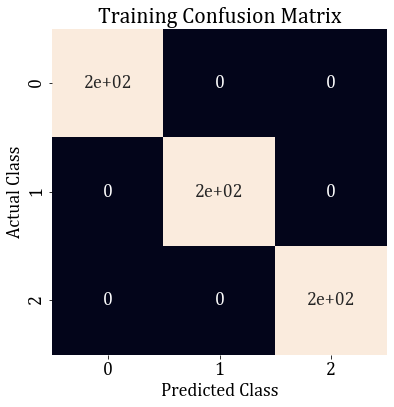
\includegraphics[scale=0.6]{images/1B/1b_conf_mat_knn_train.png}
    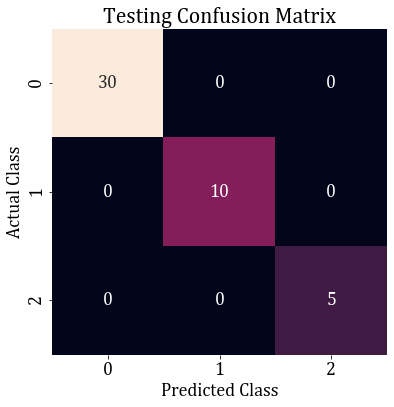
\includegraphics[scale=0.6]{images/1B/1b_conf_mat_knn_test.png}
    \caption{Confusion matrix for $k=1$, for Train and Test data on left and right respectively }
    \label{fig:1b_cm_KNN}
\end{figure}

\subsubsection{Decision Boundary plot}

\begin{figure}[H]
    \centering
    \includegraphics[scale=0.7]{images/1B/1b_KNN_decision_region.png}
    \caption{Decision boundary plot for $k=1$.}
    \label{fig:1b_decreg_KNN}
\end{figure}

\noi
The decision boundary obtained is non-linear in form and not smooth. 

\break
\subsection{Bayes Classifier, GMM, Full Covariance}
\subsubsection{Equations}
Th initialization is done as follows for each class:
\begin{itemize}
    \itemsep0em
    \item Cluster initialization is done using \tt{kmeans} clustering.
    \item The relative number of points in each cluster $N_q$ and weightage $w_q$ for each cluster is calculated.
    \item The responsibility $\gamma_{n,q}$ is then calculated, followed by mean $\mu_q$ and covariance matrix $C_q$.
\end{itemize}

\noi
The parameters are then updated sequentially through the:
\begin{itemize}
    \itemsep0em
    \item Expectation-step: $\gamma_{n,q}$ is updated.
    \item Maximization-step: $\mu_q$, $C_q$, $N_q$ and $w_q$ are updated.
\end{itemize}

\noi
The stopping criterion used is $\Delta(\text{likelihood})<\tt{tol}$. The \tt{tol} we considered is $10^{-5}$.\\

\subsubsection{Training and Validation Accuracy}
The training and validation accuracies obtained for varying $q_i$ for each class is as follows:
\begin{figure}[H]
    \centering
    \hspace{-2em}
    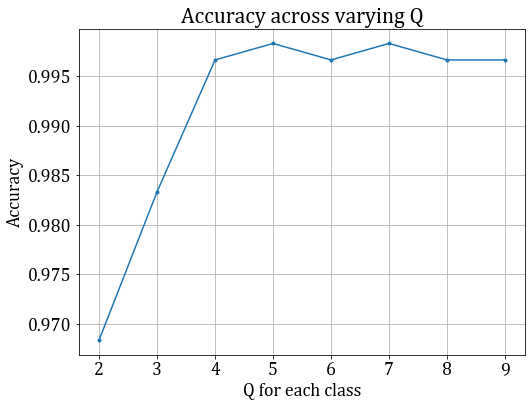
\includegraphics[scale=0.45]{images/1B/1b_full_train.png}
    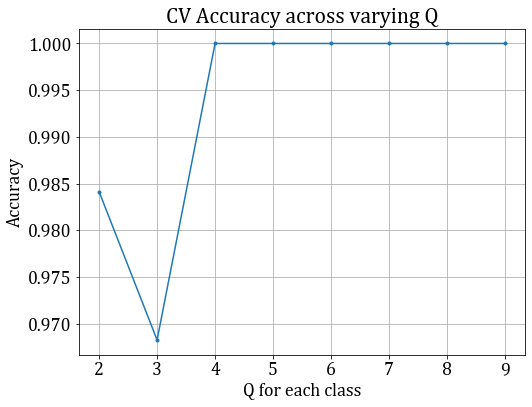
\includegraphics[scale=0.45]{images/1B/1b_full_val.png}
    \caption{Training and Validation accuracy across $q_i$, on the left and right respectively, using a GMM model with full covariance matrix.}
\end{figure}

\subsubsection{Testing Accuracy}
The testing accuracy obtained for varying $q_i$ for each class is as follows:
\begin{figure}[H]
    \centering
    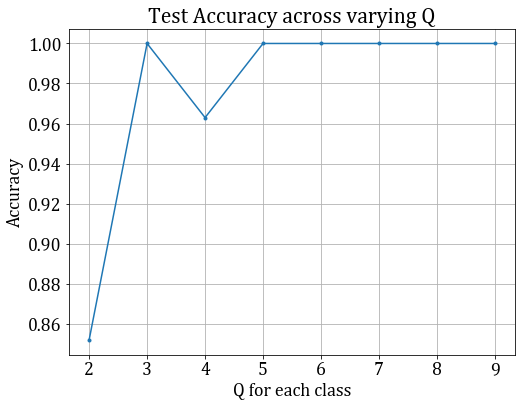
\includegraphics[scale=0.45]{images/1B/1b_full_test.png}
    \caption{Testing accuracy across $q_i$, using a GMM model with full covariance matrix.}
\end{figure}

\subsubsection{Best Model}
Based on the accuracies obtained on the training, validation and test dataset, the best $q_i$ for the three classes has been chosen as $5$. The accuracies obtained in tabular format is as follows:
\begin{table}[H]
\centering
\begin{tabular}{l l l l}
\hline
\hline
\textbf{\# Clusters/Class (Q)} & \textbf{Train Accuracy} & \textbf{Validation Accuracy} & \textbf{Test Accuracy}\\
\hline
\hline
2 & 0.968333 & 0.952381 & 0.925926 \\
3 & 0.983333 & 0.968254 & 1.000000 \\
4 & 0.996667 & 0.984127 & 1.000000 \\
\hl{5} & \hl{0.998333} & \hl{1.000000} & \hl{1.000000} \\
6 & 0.996667 & 1.000000 & 1.000000 \\
7 & 0.998333 & 1.000000 & 1.000000 \\
8 & 0.996667 & 1.000000 & 1.000000 \\
9 & 0.996667 & 1.000000 & 1.000000 \\
\hline
\end{tabular}
\caption{Variation of accuracy across hyperparameter values on the training, validation and test set using full covariance matrix GMM model on Dataset 1B. The row corresponding to the best model has been highlighted.}
\label{tab:1b_full}
\end{table}


\noi
The confusion matrix obtained for the model with $q_i=5$ are as follows:
\begin{figure}[H]
    \centering
    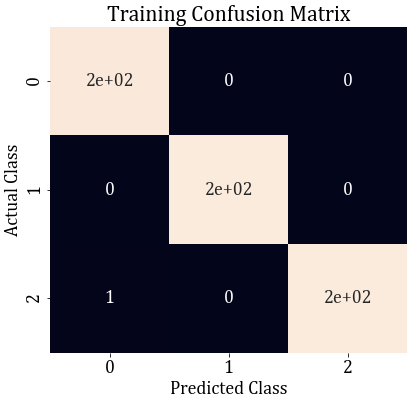
\includegraphics[scale=0.5]{images/1B/1b_full_train_conf.png}
    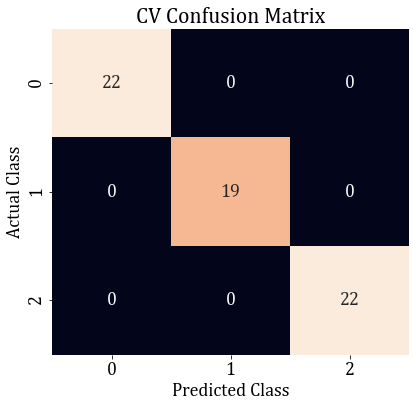
\includegraphics[scale=0.5]{images/1B/1b_full_val_conf.png}
    \caption{Confusion matrices corresponding to training and validation data, with $q_i=5$, on the left and right respectively, using GMM model with full covariance.}
\end{figure}
\vspace{-1em}
\begin{figure}[H]
    \centering
    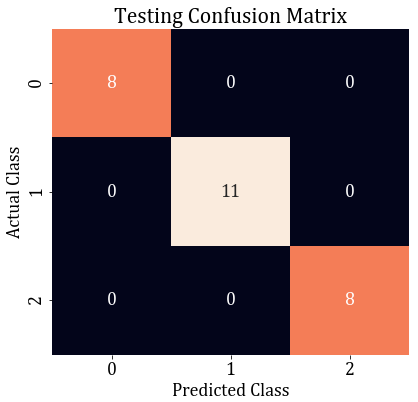
\includegraphics[scale=0.5]{images/1B/1b_full_test_conf.png}
    \caption{Confusion matrix corresponding to the testing data, with $q_i=5$, using GMM model with full covariance.}
\end{figure}

\subsubsection{Contour Maps and Decision Surfaces}
The contour maps and decision surfaces obtained, with $q_i=5$ are as follows:
\begin{figure}[H]
    \hspace{-1em}
    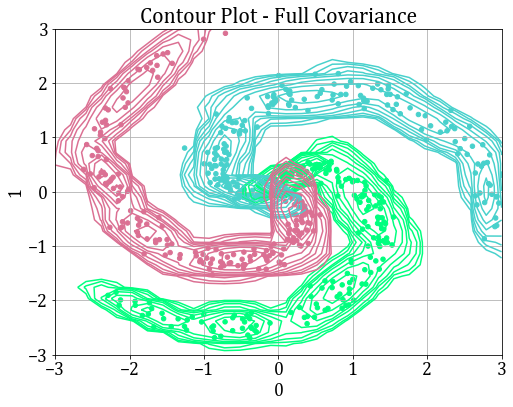
\includegraphics[scale=0.5]{images/1B/1b_full_contours.png}
    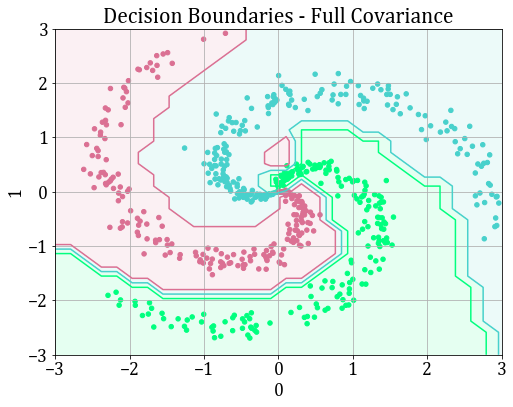
\includegraphics[scale=0.5]{images/1B/1b_full_decision_surfaces.png}
    \caption{Contour Maps, Decision Surfaces obtained for $q_i=5$, on the left and right respectively.}
\end{figure}
\vspace{-1em}
\begin{figure}[H]
    \centering
    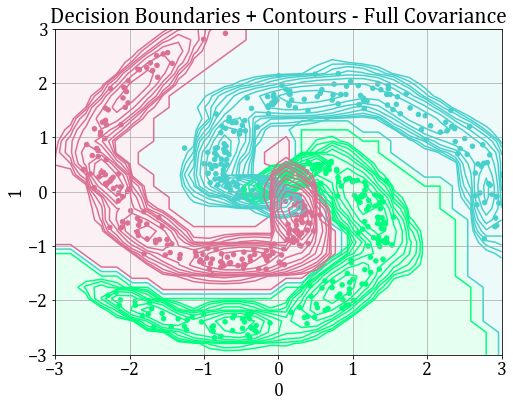
\includegraphics[scale=0.5]{images/1B/1b_full_ds_contours.png}
    \caption{Overlap plot of the decision surface and contours.}
\end{figure}

\subsection{Bayes Classifier, GMM, Diagonal covariance}
\subsubsection{Training and Validation accuracy}
Gaussian multi-modal training (with threshold of the increment in total log-likelihood functions as 0.01) with diagonal covariance matrix was used, for the number of gaussian components Q = {2,3,4,5,6,7,8,9} to estimate the parameters - $\mu_q$, $C_q$, $N_q$ and $w_q$ for each gaussian component - and predict the classes of the training data (train.csv) and cross-validation (70\% of dev.csv). The table \ref{tab:cv1b} shows the results obtained.
\begin{table}[H]
\centering
\begin{tabular}{l l l}
\hline
\hline
\textbf{\# Clusters/Class (Q)} &  \textbf{Validation Accuracy} &  \textbf{Training Accuracy}  \\
\hline
\hline
2 & 0.873 & 0.9166\\
3 & 0.920 & 0.976\\
4 & 0.968 & 0.9966\\
\hl{5} & \hl{0.984} & \hl{1.0}\\
6 & 0.984 & 0.986\\
7 & 0.984 & 0.991\\
8 & 0.984 & 0.9916\\
9 & 0.984 & 0.9916\\
\hline
\end{tabular}
\caption{Variation of accuracy across hyperparameter values on the validation data using the GMM model with diagonal covariance matrix on Dataset 1B. The row corresponding to the best model has been highlighted.}
\label{tab:cv1b}
\end{table}



\vspace{-2em}
\begin{figure}[H]
    \centering
    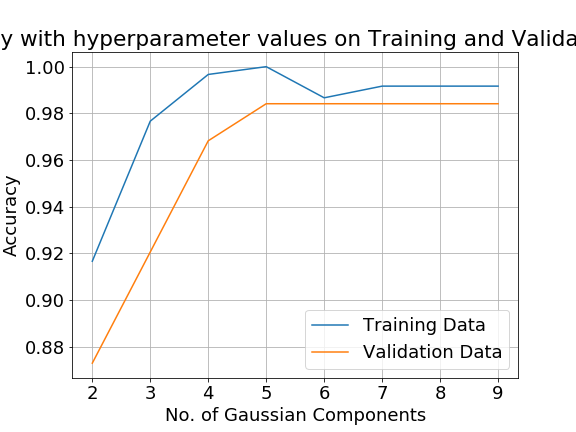
\includegraphics[scale=0.5]{images/1B/acc_1b.png}
    \caption{Training and Validation accuracy across $q_i$, using the GMM model with diagonal covariance matrix on Dataset 1B}
    \label{fig:acc1bGMMdiag}
\end{figure}

\subsubsection{Best model output}
As we can see in the tables and \autoref{fig:acc1bGMMdiag}, the best accuracy is when the number of Gaussian components is 5. Using the parameters of the model for 5 gaussian components and predicting for the test dataset (30\% of \tt{dev.csv}), the accuracy obtained was \textbf{100.0}.\\
The confusion matrices for the training and test datasets using the best model is \autoref{fig:conf_1b_diag}.
\begin{figure}[H]
    \centering
    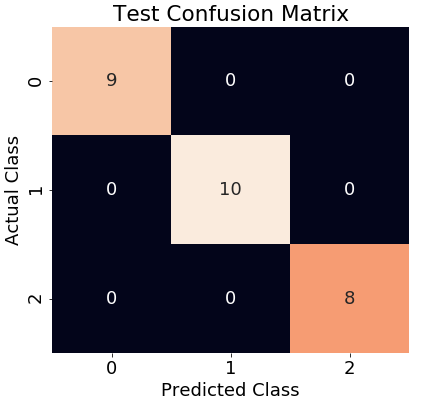
\includegraphics[scale=0.45]{images/1B/conf_test1b.png}
    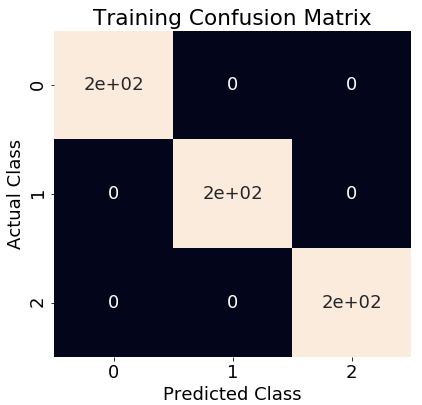
\includegraphics[scale=0.45]{images/1B/conf_train1b.png}
    \caption{Confusion matrices for data 1B - diagonal covariance matrices}
    \label{fig:conf_1b_diag}
\end{figure}

\subsubsection{Decision surface}
The decision surface plot and the contour plot for the best model is \autoref{fig:dec1bGMMdiag}. As we can see in the decision region plots, the contours follow the non-linear shape of the data. The level curves are ellipses parallel to the coordinate access, since diagonal covariance matrices were used. \autoref{fig:dec1bGMMdiag}.
\begin{figure}[H]
    \centering
    \hspace{4em}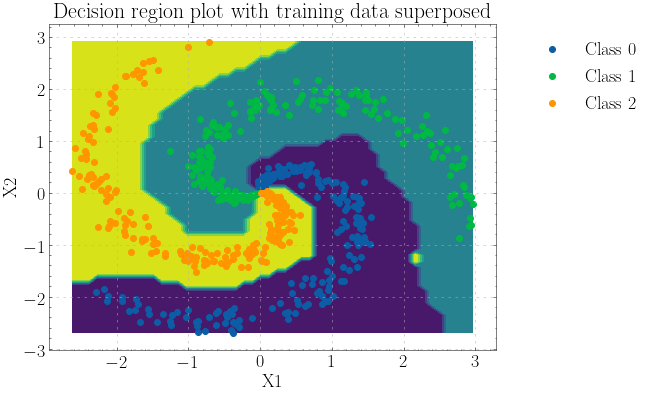
\includegraphics[scale=0.5]{images/1B/decisionReg_ds2.png}
    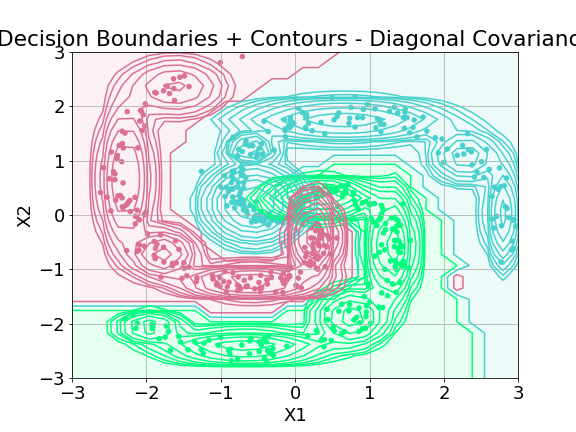
\includegraphics[scale=0.5]{images/1B/contour1b.png}
    \caption{Decision region plot for Bayesian GMM model using diagonal covariance matrix and 5 gaussian components on dataset 1B}
    \label{fig:dec1bGMMdiag}
\end{figure}

\subsection{Bayes Classifier with KNN}
\subsubsection{Mathematical Formulation}
While the main principle remains the same as discussed in \autoref{naive-bayes}, we now use non-parametric methods to evaluate the class conditional probability $p(\vec{x}|y_{i})$.\\

\noi
Suppose the number of data points in the hyper-volume v around $\vec{x}$ be N, the number of data point corresponding to class i be $N_i$, then:

\begin{equation}
    p(\vec{x}|y_{i})=\frac{N_{i}}{N*V}
\end{equation}

The probability density can be estimated in two ways :
\begin{itemize}
    \itemsep0em
    \item Specifying the volume V, number of point $N_i$ and $N$ are calculated
    \item Specifying N, the volume V and $N_i$ are calculated. Here, the radius of hyper sphere is the distance of the point belonging to N farthest from $\vec{x}$, this is called KNN method.  
\end{itemize}

\noi
For this case, we use the KNN method to evaluate the class conditional probability densities.\\
The class label $i$ that maximizes \autoref{eqn nb} is chosen as the label for $\vec{x}$. 

\subsubsection{Model Performance for varying values of \textit{k}}
The model is tested for $k=10$ and $k=20$. The accuracy table and confusion matrix are as follows:
\def\arraystretch{1.25}
\begin{table}[H]
\centering
\begin{tabular}{l l l l l}
\hline
\hline
\textbf{k-value} & \textbf{Train accuracy} & \textbf{validation accuracy} & \textbf{Test Accuracy}\\
\hline
\hline
10 & 99.1667 & 100.0 & 95.5556 \\
20 & 98.6667 & 100.0 & 93.3333 \\
\hline
\end{tabular}
\caption{Accuracy table for dataset 2A - Bayes Classifier with knn}
\end{table}

\noi
Since the accuracy is higher for $k=10$, it is used to further evaluate the confusion matrix and decision boundary plot. 

\begin{figure}[H]
    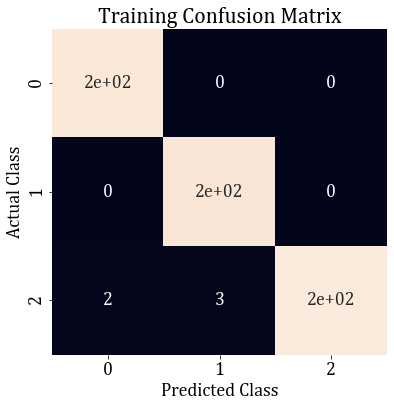
\includegraphics[scale=0.6]{images/1B/1b_conf_mat_nb_train.png}
    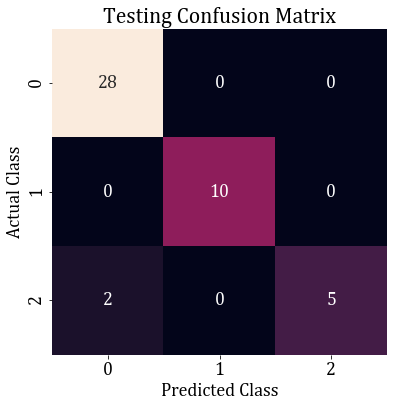
\includegraphics[scale=0.6]{images/1B/1b_conf_mat_nb_test.png}
    \caption{Confusion matrices for $k=10$, for train data and test data on left and right respectively.}
    \label{fig:1b_cm_nb}
\end{figure}

\subsubsection{Decision boundary plot}
\begin{figure}[H]
    \centering
    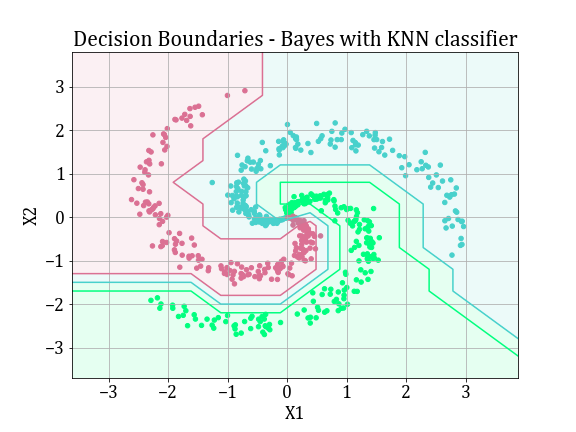
\includegraphics[scale=0.7]{images/1B/1b_nb_decision_region.png}
    \caption{Decision boundary for $k=10$}
    \label{fig:1b_decreg_nb}
\end{figure}
While the shape of decision boundary is almost similar as \autoref{fig:1b_decreg_KNN}, there are still some differences, especially near the edges.

\break
\section{Dataset 2A}
\subsection{Bayes Classifier, GMM, Full Covariance}
\subsubsection{Training and Validation Accuracy}
The training and validation accuracies obtained for varying $q_i$ for each class is as follows:
\begin{figure}[H]
    \hspace{-2em}
    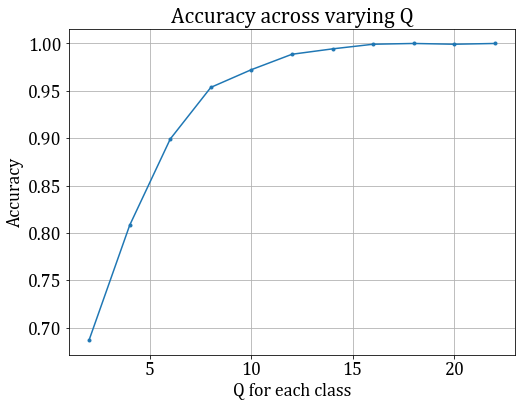
\includegraphics[scale=0.5]{images/2A/2A_full_train_acc.png}
    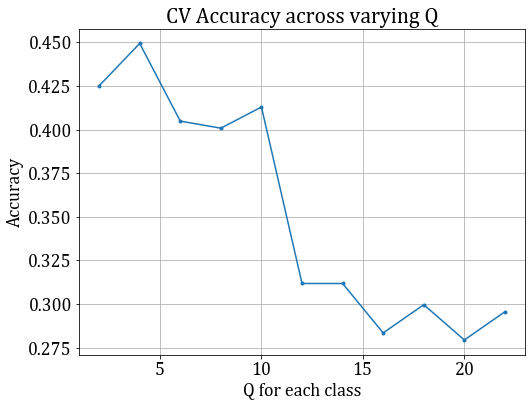
\includegraphics[scale=0.5]{images/2A/2A_full_val_acc.png}
    \caption{Training and Validation accuracy across $q_i$, on the left and right respectively}
\end{figure}

\subsubsection{Testing Accuracy}
The testing accuracy obtained for varying $q_i$ for each class is as follows:
\begin{figure}[H]
    \centering
    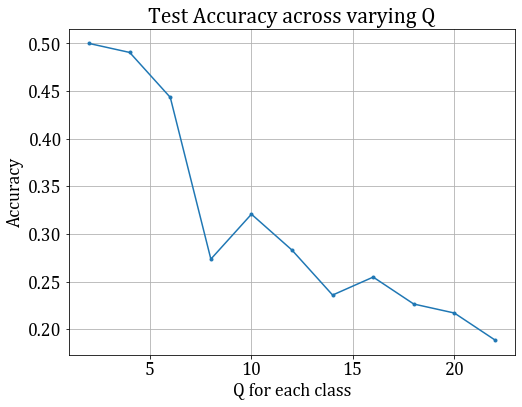
\includegraphics[scale=0.5]{images/2A/2A_full_test_acc.png}
    \caption{Testing accuracy across $q_i$}
\end{figure}

\subsubsection{Best Model}
Based on the accuracies obtained on the training, validation and test dataset, the best $q_i$ for the three classes has been chosen as $4$. The accuracies obtained in tabular format is as follows:
\begin{table}[H]
\centering
\begin{tabular}{l l l l l}
\hline
\hline
\textbf{\# Clusters/Class (Q)} & \textbf{Train Accuracy} & \textbf{Validation Accuracy} & \textbf{Test Accuracy} & \textbf{Sum(Train,Validation)} \\
\hline
\hline
2 & 0.687805 & 0.449393 & 0.462264 & 1.137198 \\
3 & 0.748780 & 0.461538 & 0.377358 & 1.210319 \\
4 & 0.800000 & 0.506073 & 0.386792 & 1.306073 \\
5 & 0.856911 & 0.485830 & 0.339623 & 1.342741 \\
\hl{6} & \hl{0.908130} & \hl{0.449393} & \hl{0.396226} & \hl{1.357523} \\
7 & 0.926016 & 0.384615 & 0.396226 & 1.310632 \\
8 & 0.957724 & 0.352227 & 0.349057 & 1.309950 \\
9 & 0.969919 & 0.380567 & 0.405660 & 1.350486 \\
10 & 0.980488 & 0.331984 & 0.320755 & 1.312472 \\
11 & 0.982927 & 0.336032 & 0.301887 & 1.318959 \\
12 & 0.982114 & 0.327935 & 0.254717 & 1.310049 \\
13 & 0.993496 & 0.279352 & 0.254717 & 1.272848 \\
14 & 0.994309 & 0.331984 & 0.283019 & 1.326293 \\
15 & 0.995935 & 0.267206 & 0.216981 & 1.263141 \\
16 & 0.995935 & 0.336032 & 0.283019 & 1.331967 \\
17 & 0.997561 & 0.279352 & 0.235849 & 1.276913 \\
18 & 1.000000 & 0.259109 & 0.235849 & 1.259109 \\
19 & 0.997561 & 0.263158 & 0.179245 & 1.260719 \\
20 & 0.999187 & 0.275304 & 0.179245 & 1.274491 \\
21 & 0.999187 & 0.275304 & 0.160377 & 1.274491 \\
22 & 1.000000 & 0.336032 & 0.273585 & 1.336032 \\
\hline
\end{tabular}
\caption{Variation of accuracy across hyperparameter values on the training, validation and test set using the GMM model with full covariance matrix on Dataset 2A. The row corresponding to the best model has been highlighted.}
\label{tab:1b_full}
\end{table}



\noi
The confusion matrix obtained for the model with $q_i=4$ are as follows:
\begin{figure}[H]
    \centering
    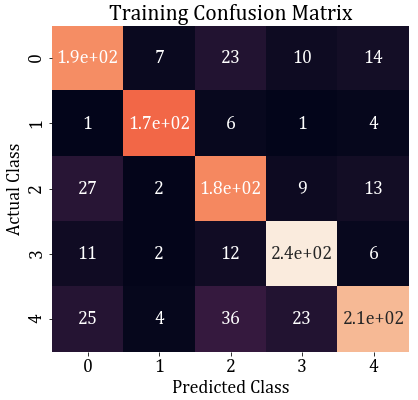
\includegraphics[scale=0.5]{images/2A/2A_full_train_conf.png}
    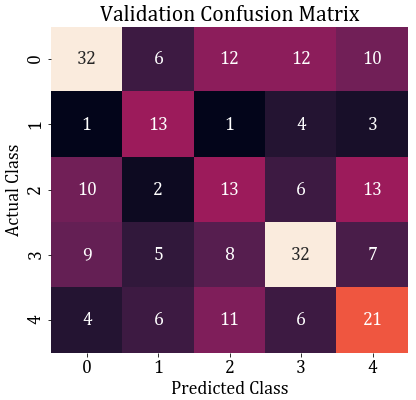
\includegraphics[scale=0.5]{images/2A/2A_full_val_conf.png}
    \caption{Training and Validation confusion matrices for the best model with $q_i=4$, on the left and right respectively}
\end{figure}

\begin{figure}[H]
    \centering
    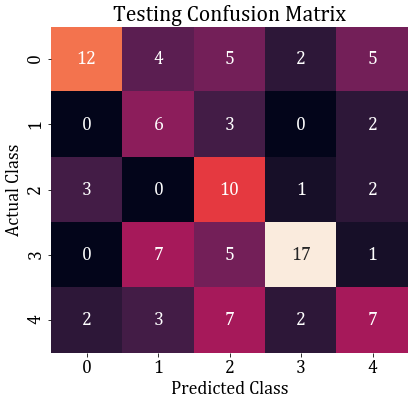
\includegraphics[scale=0.5]{images/2A/2A_full_test_conf.png}
    \caption{Testing confusion matrix for the best model with $q_i=4$.}
\end{figure}

\noi
In addition to just taking the same number of clusters for all classes, a parameter sweep was done to identify the best combination of cluster numbers for the dataset. The accuracies obtained from the parameter sweeps are as follows:
\begin{figure}[H]
    \centering
    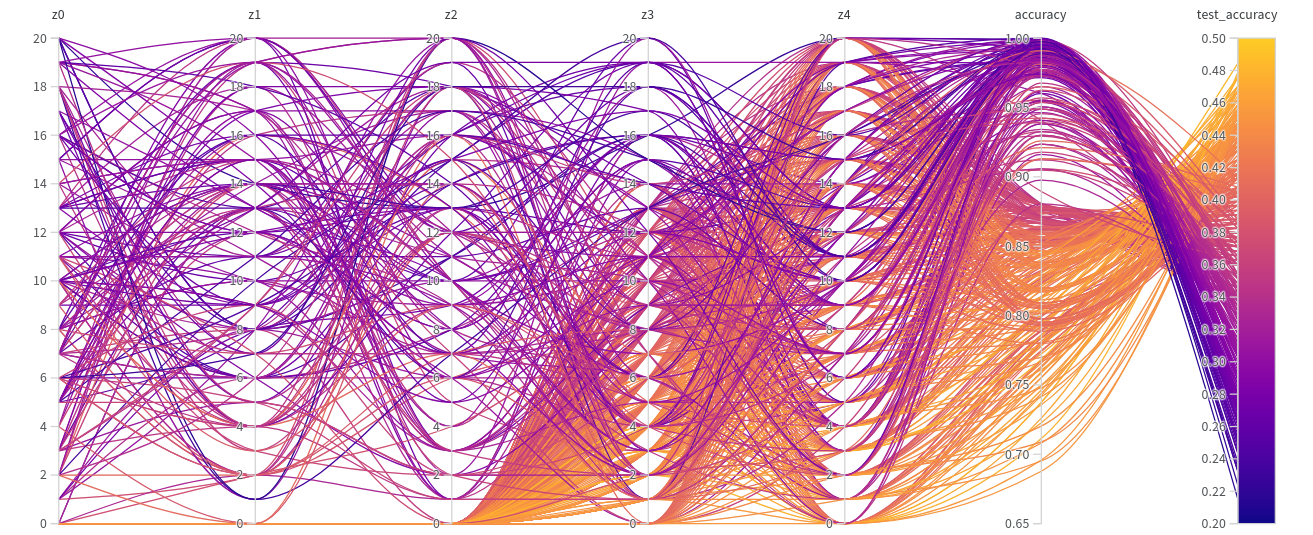
\includegraphics[scale=0.35]{images/2A/2a_parameter_sweep.png}
    \caption{Parameter Sweep Results for the dataset 2A.}
\end{figure}

\noi
From the graph above, the parameter combination that resulted in the best validation accuracy is:
\begin{itemize}
    \itemsep0em
    \item $q_1: 2$
    \item $q_2: 2$
    \item $q_3: 2$
    \item $q_4: 6$
    \item $q_5: 3$
\end{itemize}

\noi
The accuracies obtained are as follows:
\begin{itemize}
    \itemsep0em
    \item Training accuracy: 0.7853658536585366
    \item Validation accuracy: 0.4939271255060729
    \item Testing accuracy: 0.46226415094339623
\end{itemize}

\noi
From the results above, we can see that the validation accuracy is higher in this case, however, the train and test accuracies are low.\\

\noi
The confusion matrices obtained are as follows:
\begin{figure}[H]
    \centering
    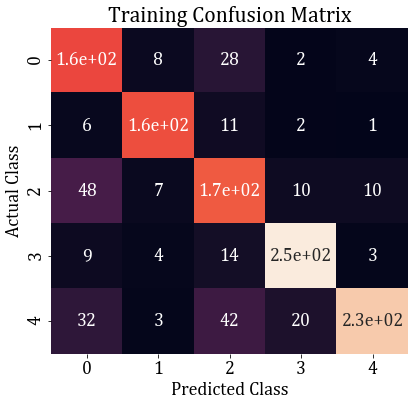
\includegraphics[scale=0.5]{images/2A/2a_full_cross_train.png}
    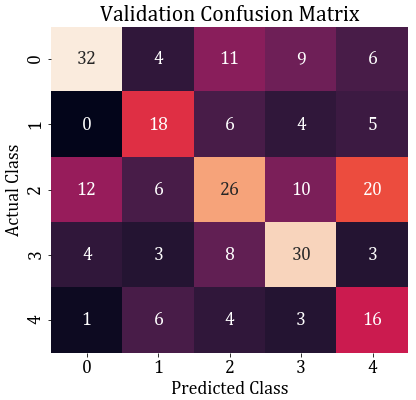
\includegraphics[scale=0.5]{images/2A/2a_full_cross_val.png}
    \caption{Training and Validation confusion matrices for the model with varying $q_i$, on the left and right respectively}
\end{figure}

\begin{figure}[H]
    \centering
    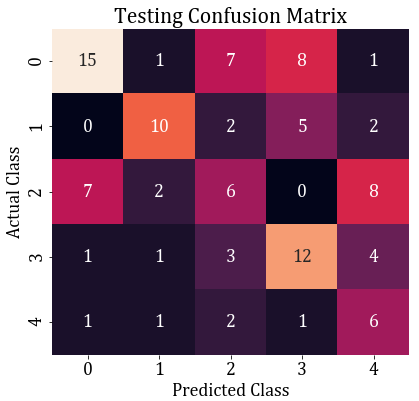
\includegraphics[scale=0.5]{images/2A/2a_full_cross_test.png}
    \caption{Testing confusion matrix for the model with varying $q_i$.}
\end{figure}


\subsection{Bayes Classifier, GMM, Diagonal covariance}
\subsubsection{Training and Validation Accuracy}
The accuracy obtained on training the data 2A on GMM model with diagonal covariance matrix is as in \autoref{tab:acc2a}.
\begin{table}[H]
\centering
\begin{tabular}{l l l l l}
\hline
\hline
\textbf{\# Clusters/Class (Q)} & \textbf{Train Accuracy} & \textbf{Validation Accuracy} & \textbf{Test Accuracy} \\
\hline
\hline
16 & 76.9106 & 46.9636 & 42.4528 \\
4 & 57.1545 & 46.9636 & 36.7925 \\
20 & 82.9268 & 45.7490 & 41.5094 \\
14 & 75.5285 & 44.9393 & 35.8491 \\
10 & 68.6179 & 44.5344 & 41.5094 \\
8 & 67.9675 & 42.5101 & 33.0189 \\
6 & 62.8455 & 41.2955 & 41.5094 \\
22 & 83.8211 & 39.6761 & 40.5660 \\
18 & 78.9431 & 39.6761 & 41.5094 \\
12 & 73.9024 & 39.2713 & 40.5660 \\
2 & 49.5122 & 38.0567 & 33.9623 \\
\hline
\end{tabular}
\caption{Accuracy across hyperparameter values on the training, validation and test dataset using the GMM model with diagonal covariance matrix on Dataset 2A. }
\label{tab:acc2a}
\end{table}



\noi
The training and validation accuracies obtained for varying $q_i$ for each class is as follows:
\begin{figure}[H]
    \hspace{-2em}
    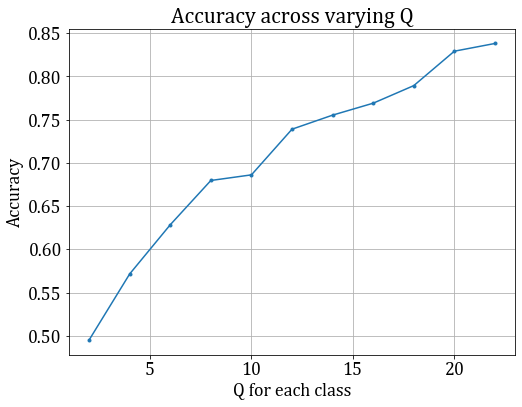
\includegraphics[scale=0.5]{images/2A/2A_diag_train_acc.png}
    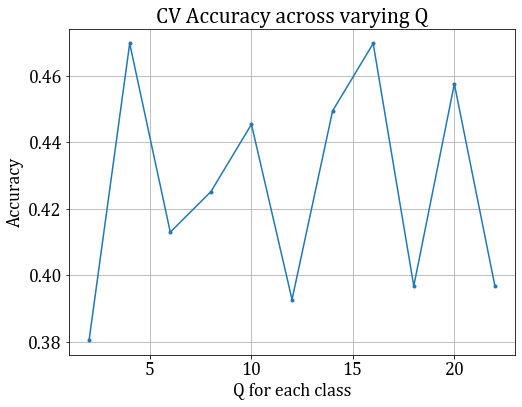
\includegraphics[scale=0.5]{images/2A/2A_diag_val_acc.png}
    \caption{Training and Validation accuracy across $q_i$, on the left and right respectively}
\end{figure}

\subsubsection{Testing Accuracy}
The testing accuracy obtained for varying $q_i$ for each class is as follows:
\begin{figure}[H]
    \centering
    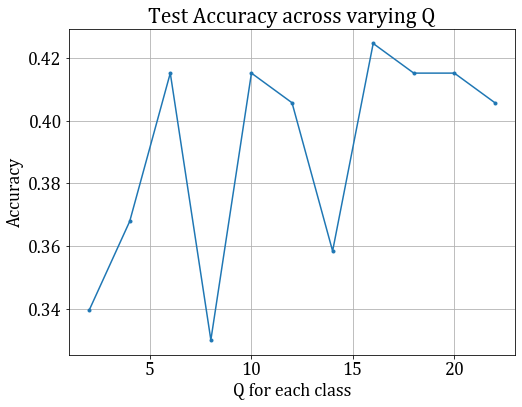
\includegraphics[scale=0.5]{images/2A/2A_diag_test_acc.png}
    \caption{Testing accuracy across $q_i$}
\end{figure}

\subsubsection{Best model on test data}
The highest accuracy on validation dataset is for 16 gaussian components. Applying this model to predict the test data, we get an accuracy of \textbf{42.45\%}. The confusion matrices for this model on training, validation and test data is as follows:
\begin{figure}[H]
    \centering
    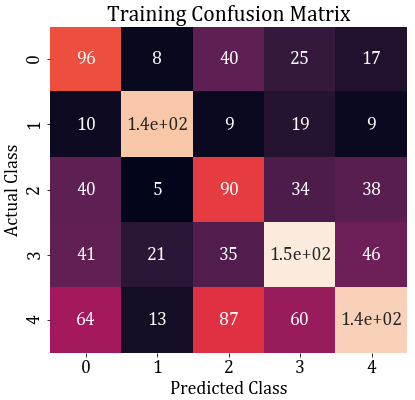
\includegraphics[scale=0.5]{images/2A/2A_diag_train_conf.png}
    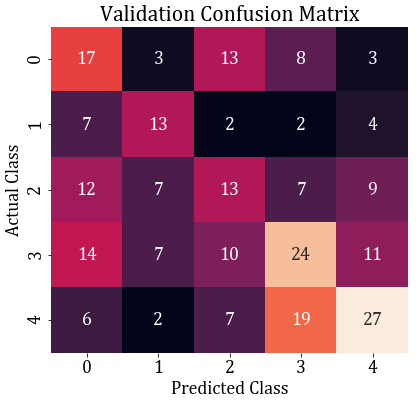
\includegraphics[scale=0.5]{images/2A/2A_diag_val_conf.png}
    \caption{Training and Validation confusion matrices for the best model with $q_i=16$, on the left and right respectively}
\end{figure}

\begin{figure}[H]
    \centering
    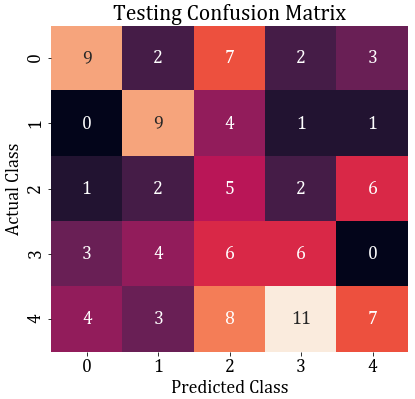
\includegraphics[scale=0.5]{images/2A/2A_diag_test_conf.png}
    \caption{Testing confusion matrix for the best model with $q_i=16$.}
\end{figure}


\break
\section{Dataset 2B}
The varying length classification is done as follows:
\begin{itemize}
    \itemsep0em
    \item Each image has a $36\times 23$ feature parameters.
    \item Each of these $36$ rows are considered as features and a GMM (full covariance/diagonal covariance) is fit on each of the features.
    \item The Expectation-step and Maximization-step are performed on the data, as is in case of static length pattern.
    \item For each of the data points, 
    \begin{equation}
    p (X|\lambda_i ) = \prod_{t=1}^T p(x_t|\lambda_i) = \prod_{t=1}^T \sum_{q=1}^Q w_{iq}\mathcal{N}(x_t|\mu_{iq}, \Sigma_{iq})
    \end{equation}
    is calculated to perform classification.
    \item In order to circumvent the problem associated with floating point precession, the Gaussian probabilities for each of the 36 features were normalized across classes and the product was then performed.
    \item The data point is then allotted to the class that has the maximum probability.
\end{itemize}

\subsection{Bayes Classifier, GMM, Full Covariance}
\subsubsection{Training Accuracies}
The class-wise training accuracy obtained for varying $q$'s is as follows:
\begin{table}[H]
\centering
\begin{tabular}{l l l l l l}
\hline
\hline
\textbf{Q} & \textbf{Coast} & \textbf{Highway} & \textbf{Mountain} & \textbf{Open Country} & \textbf{Tall Building} \\
\hline
\hline
3 & 99.601594 & 100 & 99.616858 & 100 & 100 \\
5 & 100 &  100 &  100 &  100 &  100 \\
14 & 100 & 100 & 100 & 100 & 100 \\
20 & 100 & 100 & 100 & 100 & 100 \\
\hline
\end{tabular}
\caption{Accuracy across hyperparameter values on the training dataset using the GMM model with full covariance matrix on Dataset 2B.}
\label{tab:1b_full}
\end{table}


\subsubsection{Dev Accuracies}
The class-wise accuracy obtained on the dev dataset, for varying $q$'s is as follows:
\begin{table}[H]
\centering
\begin{tabular}{l l l l l l}
\hline
\hline
\textbf{Q} & \textbf{Coast} & \textbf{Highway} & \textbf{Mountain} & \textbf{Open Country} & \textbf{Tall Building} \\
\hline
\hline
3 & 86.301370 & 46.153846 & 73.333333 & 69.512195 & 90.140845 \\
5 & 78.082192 & 32.692308 & 54.666667 & 63.414634 & 91.549296 \\
14 & 80.821918 & 0.000000 & 45.333333 & 40.243902 & 92.957746 \\
20 & 80.821918 & 0.000000 & 45.333333 & 40.243902 & 92.957746\\
\hline
\end{tabular}
\caption{Accuracy across hyperparameter values on the dev dataset using the GMM model with full covariance matrix on Dataset 2B.}
\label{tab:2b_full_dev}
\end{table}


\noi
From the tables above, we see that the maximum accuracy for the classes: coast, highway, mountain and open country are for 3 GMMs per feature. However, the accuracy for the class tall buildings increases with increasing number of GMM components.

\subsubsection{Best Model}
The highest accuracy on validation dataset is for 3 gaussian components for each feature. The overall training accuracy for the best model chosen is: 99.83739837398375\\

\noi
Applying this model to predict the test data, we get an accuracy of \textbf{74.50\%}. The confusion matrices for this model on training, validation and test data is as follows:
\begin{figure}[H]
    \centering
    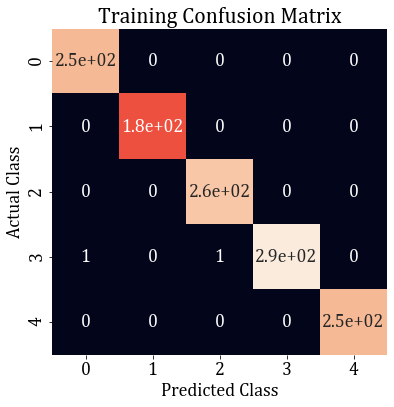
\includegraphics[scale=0.6]{images/2B/2B_full_train_conf.png}
    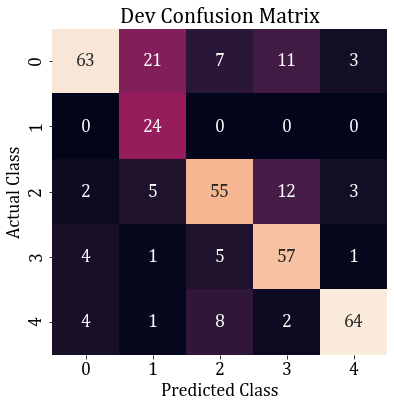
\includegraphics[scale=0.6]{images/2B/2B_full_dev_conf.png}
    \caption{Training and Dev confusion matrices for the best model with $q_i=3$, on the left and right respectively}
\end{figure}

\subsection{Bayes Classifier, GMM, Diagonal Covariance}
\subsubsection{Training Accuracies}
The class-wise training accuracy obtained for varying $q$'s is as follows:
\begin{table}[H]
\centering
\begin{tabular}{l l l l l l}
\hline
\hline
\textbf{Q} & \textbf{Coast} & \textbf{Highway} & \textbf{Mountain} & \textbf{Open Country} & \textbf{Tall Building} \\
\hline
\hline
3 & 85.657371 & 87.912088 & 88.505747 & 90.592334 & 88.755020\\
5 & 92.828685 & 95.604396 & 94.636015 & 95.121951 & 95.582329 \\
14 & 99.203187 & 100 & 100 & 100 & 99.196787 \\
20 & 100 & 100 & 100 & 100 & 99.598394 \\
\hline
\end{tabular}
\caption{Accuracy across hyperparameter values on the training dataset using the GMM model with diagonal covariance matrix on Dataset 2B.}
\label{tab:2B_diag_train}
\end{table}



\subsubsection{Dev Accuracies}
The class-wise accuracy obtained on the dev dataset, for varying $q$'s is as follows:
\begin{table}[H]
\centering
\begin{tabular}{l l l l l l}
\hline
\hline
\textbf{Q} & \textbf{Coast} & \textbf{Highway} & \textbf{Mountain} & \textbf{Open Country} & \textbf{Tall Building} \\
\hline
\hline
3 & 61.643836 & 65.384615 & 70.666667 & 78.048780 & 76.056338 \\
5 & 68.493151 & 69.230769 & 77.333333 & 74.390244 & 77.464789 \\
14 & 78.082192 & 48.076923 & 66.666667 & 74.390244 & 87.323944 \\
20 & 75.342466 & 46.153846 & 73.333333 & 71.951220 & 90.140845 \\
\hline
\end{tabular}
\caption{Accuracy across hyperparameter values on the training dataset using the GMM model with diagonal covariance matrix on Dataset 2B.}
\label{tab:1b_full}
\end{table}


\noi
From the tables above, we see that the maximum accuracy for the classes: highway, mountain and open country are for 5 GMMs per feature. However, the accuracy for the class tall buildings increases with increasing number of GMM components and the maximum accuracy for the class coast is obtained at 14 GMMs per feature.

\subsubsection{Best Model}
The highest accuracy on validation dataset is for 5 gaussian components for each feature. The overall training accuracy for the best model chosen is: 94.71544715447155\\

\noi
Applying this model to predict the test data, we get an accuracy of \textbf{73.65\%}. The confusion matrices for this model on training, validation and test data is as follows:
\begin{figure}[H]
    \centering
    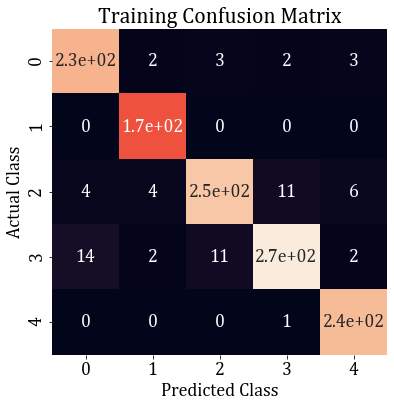
\includegraphics[scale=0.55]{images/2B/2B_diag_train_conf.png}
    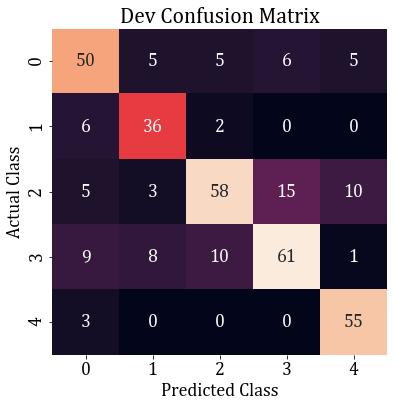
\includegraphics[scale=0.55]{images/2B/2B_diag_dev_conf.png}
    \caption{Training and Dev confusion matrices for the best model with $q_i=5$, on the left and right respectively}
\end{figure}

\subsection{Inference}
From \autoref{tab:2B_full_train}, \autoref{tab:2B_full_dev}, \autoref{tab:2B_diag_train} and \autoref{tab:2B_diag_dev}, we can observe the follows:
\begin{itemize}
    \itemsep0em
    \item The training accuracy increases as the number of components per feature increases irrespective of the type of covariance matrix.
    \item For the classes: Coast and Tall Building, full covariance models better fit the data than the diagonal covariance models. This indicates that the features have variations in directions that aren't parallel to the coordinate axis. 
    \item For the classes: highway, mountain and open country, diagonal covariance models better fit the data. Additionally we also note that that accuracy doesn't increase indiscriminately as a function of $q_i$, but that it peaks at an intermediate value. This could mean that the features have variations in the direction parallel to the coordinate axis and that the complexity of the data is best explained by an intermediate number of components per feature.
\end{itemize}

\end{document}
